%----------------------------------------------------------------------------------------------
%-----------------------------------     4 Grenzwerte     -------------------------------------
%----------------------------------------------------------------------------------------------
\section{Grenzwerte}

%----------------------------------------------------------------------------------------------
%-----------------------     4.1 Links- / Rechtsseitiger Grenzwert     ------------------------
%----------------------------------------------------------------------------------------------
\subsection{Links- / Rechtsseitiger Grenzwert}{55}

Eine kritische Stelle $x_0$ kann von links und rechts angen"ahert werden.
		
\renewcommand{\arraystretch}{1.7}
\begin{tabular}{ll}
	Linksseitiger Grenzwert: 	& $\lim\limits_{x \to x_0^-} f(x) = g^-$ \\
	Rechtsseitiger Grenzwert: 	& $\lim\limits_{x \to x_0^+} f(x) = g^+$ \\
\end{tabular}
\renewcommand{\arraystretch}{1}
\vspace{0.1cm}

\begin{itemize}
	\item Wenn $g^- = g^+ = g \Rightarrow$ Konvergenz 
	\item Wenn $g^- \neq g^+ \Rightarrow$ Unbestimmte Divergenz
\end{itemize}

%----------------------------------------------------------------------------------------------
%------------------------------     4.2 Konvergenz, Divergenz     -----------------------------
%----------------------------------------------------------------------------------------------
\subsection{Konvergenz, Divergenz}{472}

\subsubsection{Konvergenz von $f(x)$ \hspace{0.3cm}\texorpdfstring{$\Rightarrow$}{→} \hspace{0.3cm}1.2 Umgebung}
		
\begin{tabular}{lll}
	$x \to \infty$ 	& Toleranzungleichung: $\vert f(x) - g \vert < \varepsilon$ 	& wenn $x > M(\varepsilon)$ \\
	$x \to -\infty$ & Toleranzungleichung: $\vert f(x) - g \vert < \varepsilon$ 	& wenn $x < m(\varepsilon)$ \\
	\\
	$x \to x_0$ 	& Toleranzungleichung:  $\vert f(x) - g \vert < \varepsilon$ 	& $ x \in \dot{U}_\delta(x_0)$ \\
\end{tabular}

		
\subsubsection{Bestimmte Divergenz von $y = f(x)$}

\begin{tabular}{lll}
	\textbf{Quadrant} &  \textbf{Kriterium}									& \textbf{Folgerung}      \\
	\midrule
	\Romannum{1}	& 	$y \to \infty$ $(x \to \infty$) 	& $y > K$ wenn $x > M(K)$ \\
	\Romannum{2}	& 	$y \to \infty$ $(x \to -\infty$) 	& $y > K$ wenn $x < m(K)$ \\
	\Romannum{3}	& 	$y \to -\infty$ $(x \to -\infty$) 	& $y < k$ wenn $x < m(k)$ \\
	\Romannum{4}	& 	$y \to -\infty$ $(x \to \infty$) 	& $y < k$ wenn $x > M(k)$ \\
	\midrule
					& 	$f(x) \to \infty$ 					& $y > K > 0$ wenn $ x \in \dot{U}_\delta(x_0)$ \\
					& 	$f(x) \to -\infty$ 					& $y < k < 0$ wenn $ x \in \dot{U}_\delta(x_0)$
\end{tabular}

%----------------------------------------------------------------------------------------------
%------------------------------------     4.3 Stetigkeit     ----------------------------------
%----------------------------------------------------------------------------------------------
\subsection{Stetigkeit}{59-63, 127}

$$ \text{Definition Stetigkeit:} \quad \lim \limits_{x \to x_0} f(x) = f(x_0) $$
Eine Funktion ist stetig, wenn der Funktionsgraph gezeichnet werden kann, ohne dass der Stift abgesetzt werden muss.

\begin{center}
	\includegraphics[width=0.98\columnwidth]{images/stetigkeit.PNG} 
\end{center}

%----------------------------------------------------------------------------------------------
%---------------------     4.4 Nullstellen bestimmen gem"ass Bolzano     ----------------------
%----------------------------------------------------------------------------------------------
\subsection{Nullstellen bestimmen gem"ass Bolzano}{12}

$f(x)$ auf Intervall $[a;b]$ stetig; $f(a)$ und $f(b)$ verschiedene Vorzeichen

\textrightarrow\ Es existiert (mindestens) eine Nullstelle $\xi$ 

\subsubsection{Bisektion  (Intervallschachtelung)}

Die Nullstelle lässt sich mittels Bisektion (Intervallschachtelung) näherungsweise berechnen:
\vspace{0.2cm}
		
\begin{tabular}{llcl}
    1. & $I_0 = [a ; b] = [a_0 ; b_0]$ gesamtes Intervall\\
    2. & $I_0$ halbieren \textrightarrow\ $m = \frac{a_0 + b_0}{2}$\\
    3. & Teil-Intervall mit Vorzeichenwechsel bestimmen:\\
       &\begin{tabular}{ll}                                             
            $\Rightarrow$ & links: $f(a) \cdot f(m) < 0$ \\
            $\Rightarrow$ & rechts: $f(a) \cdot f(m) > 0$
        \end{tabular}                                                   & & $\displaystyle{n_{min} = \log_{2}{\frac{b_0-a_0}{\varepsilon_{max}}}}$\\
    4. & Teil-Intervall mit Vorzeichenwechsel: $I_1 = [a_1 ; b_1]$ \\
    5. & Schritte 2. - 4. $n$ mal wiederholen: $I_{n+1} \in I_n$\\
    6. & $\ldots \xi \in (a;b)$ mit $f(\xi) = 0$ (Nullstelle)\\
\end{tabular}

\begin{center}
	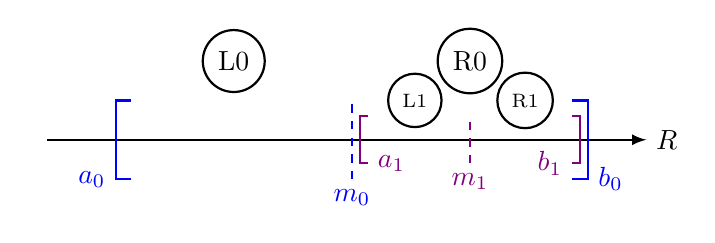
\begin{tikzpicture}
	[
		scale=1.0,
		>=latex,
		whitecircle/.style={circle, draw=black, fill=white, thick, minimum size=0.7cm},
	]

        % nodes
        \node               at (0, 0)   (O) {};             
        \node               at (8, 0)   (H) {$\mathbb{R}$}; 
        \node[whitecircle]  at (2.5, 1) (L0) {L0};
        \node[whitecircle]  at (5.5, 1) (R0) {R0};
        \node[whitecircle, minimum size=0.2cm, font=\scriptsize]  at (4.8, 0.5) (L1) {L1};
        \node[whitecircle, minimum size=0.2cm, font=\scriptsize]  at (6.2, 0.5) (R1) {R1};
        
        % main axis
        \draw[->, thick] (O) -- (H);

        % first interval (blue)
        \draw[thick, blue]          (1.2, -0.5) -- (1, -0.5) node[left] (a0) {$a_0$} -- (1, 0.5) -- (1.2, 0.5);
        \draw[thick, blue]          (6.8, -0.5) -- (7, -0.5) node[right] (b0) {$b_0$} -- (7, 0.5) -- (6.8, 0.5);
        \draw[thick, blue, dashed]  (4, -0.5) node[below] (m0) {$m_0$} -- (4, 0.5);

        % first refinement (violet)
        \draw[thick, violet]        (4.2, -0.3) node[right] (a1) {$a_1$} -- (4.1, -0.3) -- (4.1, 0.3) -- (4.2, 0.3);
        \draw[thick, violet]        (6.8, -0.3) node[left] (b1) {$b_1$} -- (6.9, -0.3) -- (6.9, 0.3) -- (6.8, 0.3);
        \draw[thick, violet, dashed](5.5, -0.3) node[below] (m1) {$m_1$} -- (5.5, 0.3);

    \end{tikzpicture}
\end{center}

%----------------------------------------------------------------------------------------------
%--------------------------------     4.5 Asymptotenbestimmung     ----------------------------
%----------------------------------------------------------------------------------------------
\subsection{Asymptotenbestimmung \hspace{0.3cm}\texorpdfstring{$\Rightarrow$}{→} \hspace{0.3cm}2.9 || 2.10}

\label{Asymptotenbestimmung}

Asymptote einer gebrochen rationalen Funktion $r(x) = \frac{P_n(x)}{Q_m(x)}$ bestimmen gem"ass: 

\renewcommand{\arraystretch}{1.3}
\begin{tabular}{l | c | c | c }
	& $m < n$ 								& $m = n$ 	& $n < m$ \\
	\hline
	$\lim\limits_{x \to \pm \infty} r(x)$ 	& $\infty$ oder $-\infty$ 		& $\frac{a_n}{b_m}$ 				& 0 \\
	Asymptote 								& ganzrat. Teil der 	        & Parallel zur $x$-Achse 		    & x-Achse \\
											& Polynomdivision			    & $y = g(x) = \frac{a_m}{b_n}$ 		& 
\end{tabular}
\renewcommand{\arraystretch}{1}
\vspace{0.4em}

\subsubsection*{Bsp. Asymptotenbestimmung}

\begin{tabular}{l}
    $ \displaystyle{ m < n:   \frac{x^2}{x-1} \quad \Rightarrow \quad x + \frac{x}{x-1} \quad \Rightarrow \quad x + \frac{x-1}{x-1} + \frac{1}{x-1} = x + 1 + \frac{1}{x-1} \quad \Rightarrow}$\\\\
    $ \displaystyle{\quad \Rightarrow \quad x + 1 + \frac{1}{x-1} \quad \Rightarrow \quad \lim\limits_{x \to \pm \infty} \frac{1}{x-1} = 0 \quad \Rightarrow \quad f(x) = x + 1 + 0}$\\\\
\end{tabular}\\
\hrule
\begin{tabular}{l}
    \\  
    $ \displaystyle{ m = n:   \frac{x}{x-1} \quad \Rightarrow \quad \frac{\frac{x}{x}}{\frac{x}{x}-\frac{1}{x}}\quad \Rightarrow \quad \lim\limits_{x \to \pm \infty} \frac{\frac{x}{x}}{\frac{x}{x}-\frac{1}{x}} = \frac{1}{1} = 1\quad \Rightarrow \quad  f(x)= 1}$\\\\
\end{tabular}\\
\hrule
\begin{tabular}{l}
    \\  
    $ \displaystyle{ n < m:   \frac{x}{x^2-1} \quad \Rightarrow \quad \frac{\frac{x}{x}}{\frac{x^2}{x}-\frac{1}{x}} \quad \Rightarrow \quad \lim\limits_{x \to \pm \infty} \frac{\frac{x}{x}}{\frac{x^2}{x}-\frac{1}{x}} = 0 \quad \Rightarrow \quad f(x) = 0}$\\
\end{tabular}

%----------------------------------------------------------------------------------------------
%--------------------------------     4.6 Spezielle Grenzwerte     ----------------------------
%----------------------------------------------------------------------------------------------
\subsection{Spezielle Grenzwerte}	

\begin{tabular}{llllll}
    $\lim\limits_{x \to \infty} (1 + \frac{a}{x})^x = \e^a$          & & $\lim\limits_{x \to 0} \frac{a^x -1}{x} = \ln(a)$ & & $\lim\limits_{x \to 0} \frac{(a+x)^\alpha -1}{x} = \alpha$ \\
    \\
    $\lim\limits_{x \to 0} \frac{\log_a(x+1)}{x} = \frac{1}{\ln(a)}$ & & $\lim\limits_{x \to 0+} x^{\sin(x)} = 1$          & & $\lim\limits_{x \to 0+} z^z = 1$	\\
    \\
    $\lim\limits_{x \to \infty} \frac{\sin(x)}{x} = 0$               & & $\lim\limits_{x \to \infty} \sqrt[x]{x} = 1$      & & $\lim\limits_{x \to 0} \frac{x}{1-\e^{-x}} = 1$ 
\end{tabular}

%----------------------------------------------------------------------------------------------
%--------------------------------     3.7 Wichtige funktion     -------------------------------
%----------------------------------------------------------------------------------------------
\subsection{Wichtige Funktionen}

\subsubsection{Exponentialfunktion}{73}
\[
\e^1 = \lim\limits_{n \to \infty} \left(1+\frac{1}{n} \right)^n \quad \quad \e^{-1} = \lim\limits_{n \to \infty} \left(1-\frac{1}{n} \right)^n \quad \quad \e^x = \lim\limits_{n \to \infty} \left(1+\frac{x}{n} \right)^n
\]
\begin{minipage}{0.45\columnwidth}
    \includegraphics[width=0.95\columnwidth]{images/exp-funktion.PNG}
\end{minipage}
\hfill
\begin{minipage}{0.5\columnwidth}
    \raggedright
    \textbf{Definitions- / Wertebereich:}
    $D_f = \mathbb{R} \rightarrow W_f = \mathbb{R^+}$ \\
    \vspace{0.4cm}
    
    \textbf{Einschliessung:}
    
    \renewcommand{\arraystretch}{1.6}
    \begin{tabular}{ll}
        $\e^x \geq 1 + x$ & f"ur $x \in \mathbb{R}$ \\
        $\e^x \leq \frac{1}{1-x}$ & f"ur $x < 1$  
    \end{tabular}
\end{minipage}
\hrule

\subsubsection{Hyperbolische Funktionen}{89}

$$ \e^x = \frac{1}{2} (\e^x - \e^{-x}) + \frac{1}{2} (\e^x + \e^{-x}) = \sinh(x) + \cosh(x) $$ 

\renewcommand{\arraystretch}{1.5}
\begin{tabular}{ll}
    $\sinh(x) = \frac{1}{2} (\e^x - \e^{-x})$ & $\mathbb{R} \to \mathbb{R}$  \\
    $\cosh(x) = \frac{1}{2} (\e^x + \e^{-x})$ & $\mathbb{R} \to [1; \infty)$ \\
    $\tanh(x)$ = $\frac{\sinh(x)}{\cosh(x)} = \frac{\frac{1}{2} (\e^x - \e^{-x})}{\frac{1}{2} (\e^x + \e^{-x})}$ & $\mathbb{R} \to (-1; 1)$ \\	

    $\vert \sinh(x) \vert < \cosh(x)$	& 
\end{tabular}
\renewcommand{\arraystretch}{1}


\subsubsection{Area-Funktionen (Umkehrung Hyperbolische. F.)}{93}

\renewcommand{\arraystretch}{1.4}
\begin{tabular}{ll}
    $\mathrm{arsinh}(x)$ & $\mathbb{R} \to \mathbb{R}$ \\
    $\mathrm{arcosh}(x)$ & $[1; \infty) \to \mathbb{R}^+_0$  \\
    $\mathrm{artanh}(x)$ & $ \vert x \vert < 1 \to \mathbb{R} $ 
\end{tabular}
\renewcommand{\arraystretch}{1}
\hrule

\subsubsection{Logarithmusfunktion}{73}
    
\begin{minipage}{0.45\columnwidth}
    \includegraphics[width=0.95\columnwidth]{images/ln-funktion.PNG}
\end{minipage}
\hfill
\begin{minipage}{0.5\columnwidth}
    \raggedright
    \textbf{Definitions- / Wertebereich:}
    $D_f = \mathbb{R^+} \rightarrow W_f = \mathbb{R}$ 
    \vspace{0.4cm}

    \textbf{Einschliessung:}
    
    $1-\frac{1}{x} \leq \ln(x) \leq x-1$
\end{minipage}

%----------------------------------------------------------------------------------------------
%----------------------------     Weiter Sachen Hier hinzufügen    ----------------------------
%----------------------------------------------------------------------------------------------